\documentclass{article}
\usepackage[utf8]{inputenc}
\usepackage[a4paper, total={6in, 8in}]{geometry}
\usepackage{graphicx}
\title{CMSC426Pj1 Report}
\author{Yizhan Ao UID: 116022064}
\author{
  Yingqiao, Gou\\
  \texttt{ygou@terpmail.umd.edu}
  \texttt{UID:115979000}
  \and
  Yizhan, Ao\\
  \texttt{josephao@umd.edu}
  \texttt{UID:116022064}
}

\date{September 22nd 2021}

\begin{document}

\maketitle

\section{Introduction}
\begin{enumerate}
    \paragraphSingle-Gaussian and Gaussian-Mixture Models are utilized in various pattern recognition tasks. The model parameters are estimated usually via Maximum Likelihood Estimation (MLE) with respect to available training data. However, if only small amount of training data is available, the resulting model will not generalize well. Loosely speaking, classification performance given an unseen test set may be poor. In this paper, we propose a novel estimation technique of the model variances. Once the variances were estimated using MLE, they are multiplied by a scaling factor, which reflects the amount of uncertainty present in the limited sample set. The optimal value of the scaling factor is based on the Kullback-Leibler criterion and on the assumption that the training and test sets are sampled from the same source distribution. In addition, in the case of GMM, the proper number of components can be determined.
\end{enumerate}

\section{Single Gaussian}
The color segmentation we need probability of the orange pixel distribution in a picture the. In Single Gaussian Color segementation there are several steps that we need to follow. 
\begin{enumerate}
    \item Read image 
    \item Convert the image to the color space 
    \item Check if the pixel is orange or not
    \item if the color threshold is orange then we collect these pixels and proceed
    \item If not we go back and redo the color and detect again on another picture. 
    \item We calculate the mean and covariance and the likelihood and posterior so we can follow the Gaussian equation and have the value of $P(Cl|x)>=r$ 
    \item Mask the image
    \item train image from training set 
    \item Train images from the testing set
\end{enumerate}
In order to find the probability distribution we need the likelihood of orange pixels of the picture. The idea is to collect all the orange pixels. Combining color thresholding and sigma to minimize the value of each color, using function $roipoly()$ we could identify the automation of clustering orange color  
\begin{itemize}
    \item $P(C_1)$ we set this probability of the pixel of being orange and the possibility that is not orange is also 0.5
    \item The $posterior(C_l|x)$ is the probabilty that the pixel is orange or not orange
    \item \begin{equation}p(C_l \mid x)=\frac{p(x \mid C_l) * p(C_l)}{\sum_{i=1}^{l} p(x \mid Ci) p(C i)}\end{equation}
    \item Posterior is directly proportional towards prior and likelihood.
    \item The thresholding is $P(C_l|x)$ which the threshold need to be higher than the confidence level
    %\item
\end{itemize}
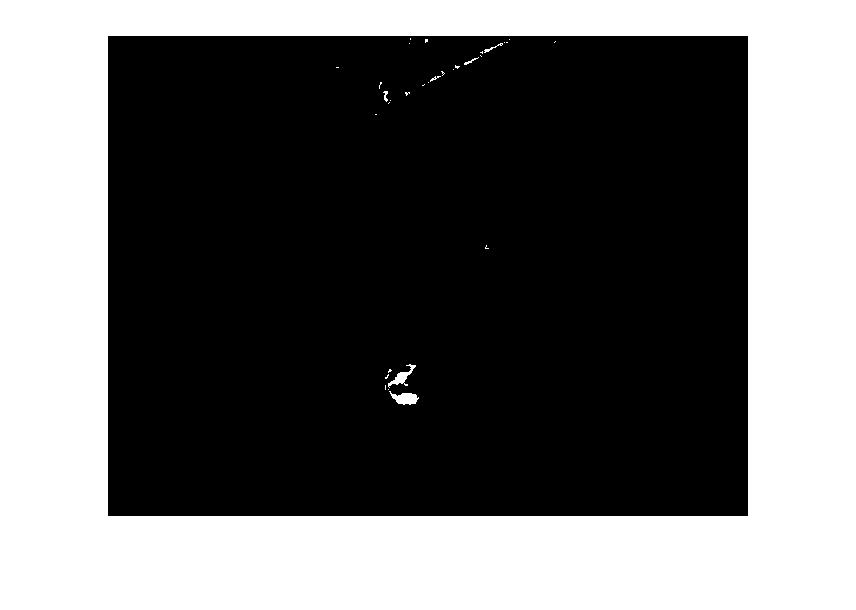
\includegraphics[scale = 0.3]{Fig1.jpg}
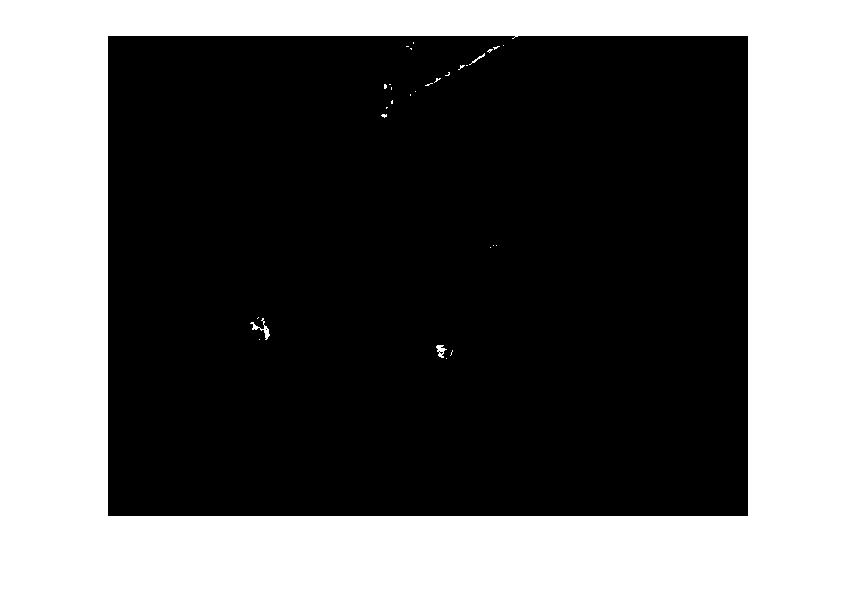
\includegraphics[scale = 0.3]{Fig2.jpg}
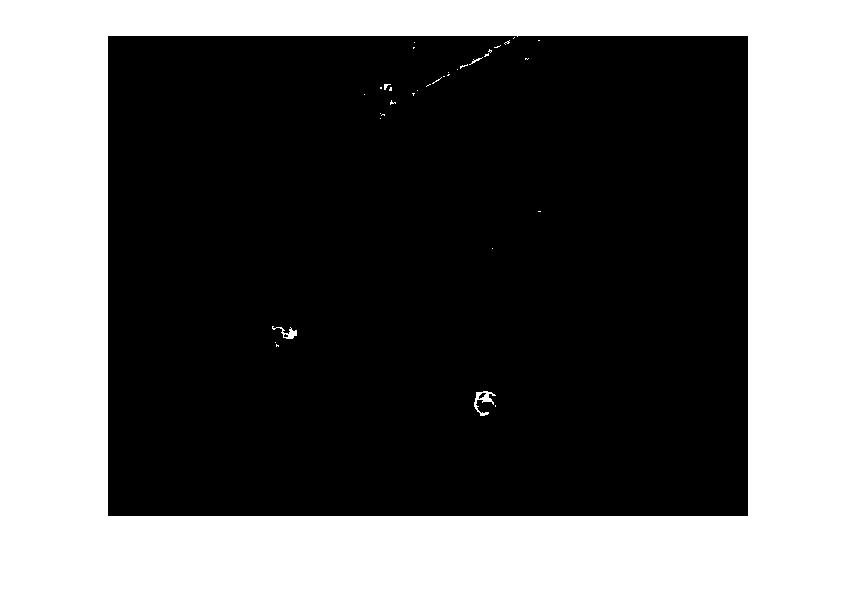
\includegraphics[scale = 0.3]{Fig3.jpg}
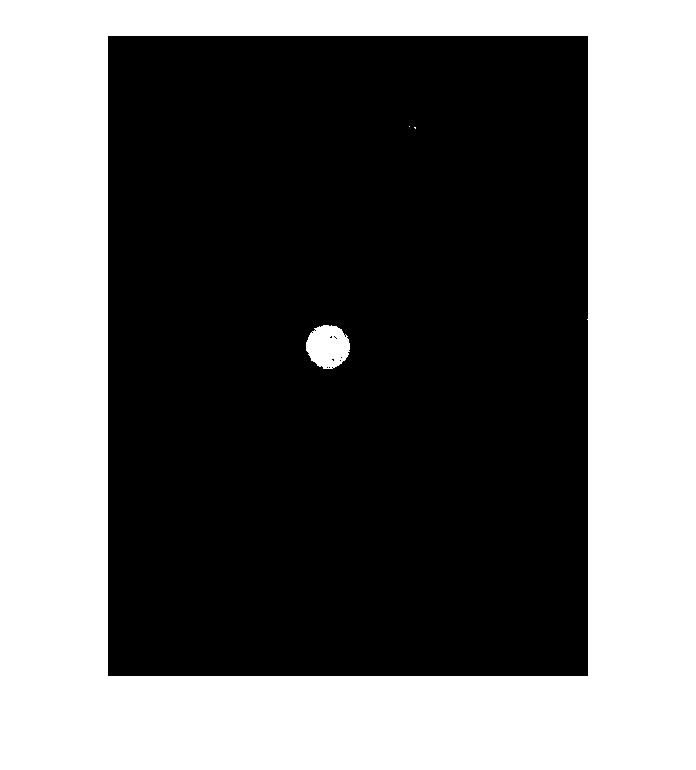
\includegraphics[scale = 0.3]{Fig4.jpg}
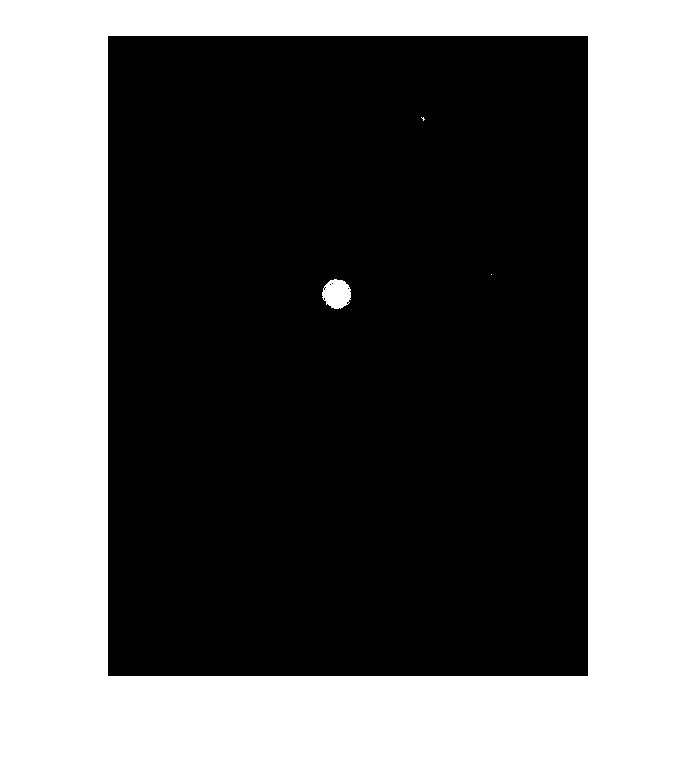
\includegraphics[scale = 0.3]{Fig5.jpg}
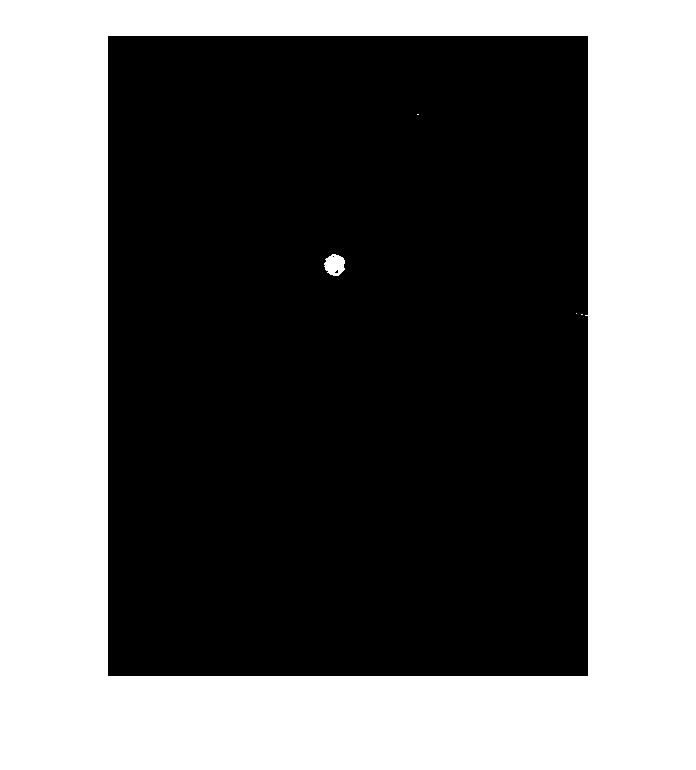
\includegraphics[scale = 0.3]{Fig6.jpg}
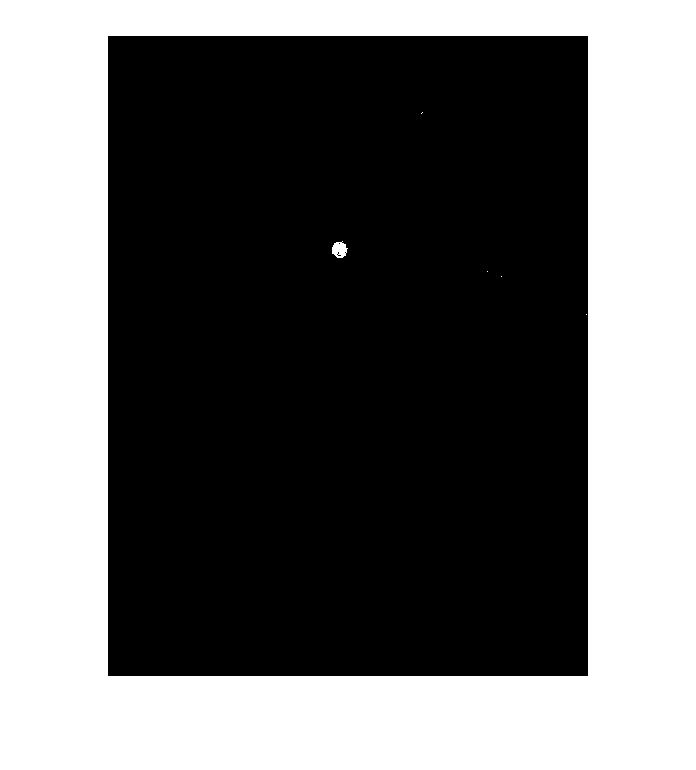
\includegraphics[scale = 0.3]{Fig7.jpg}
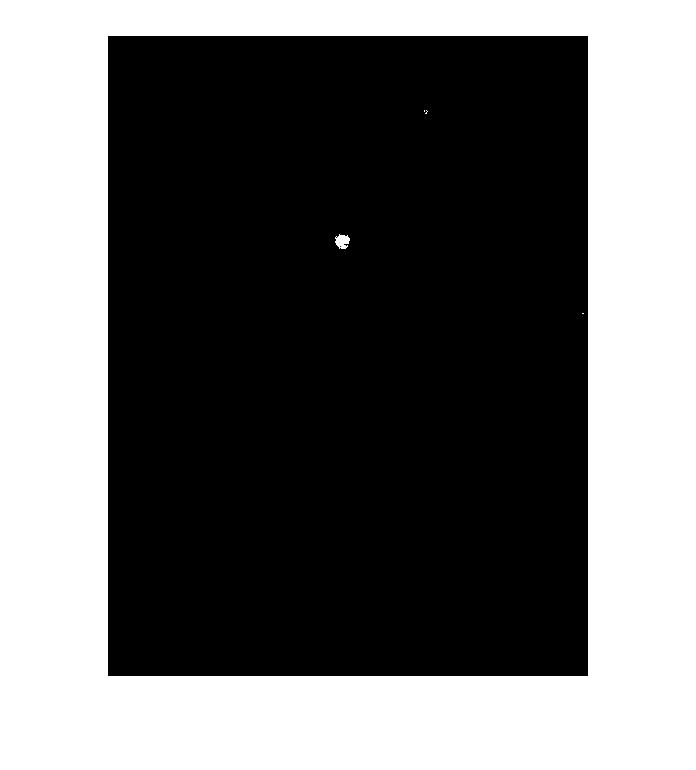
\includegraphics[scale = 0.3]{Fig8.jpg}
\textbf{Drawbacks}
\begin{itemize}
    \item Single Gaussian is very dependent from the user input. A slight change towards the training sample could make a very big difference towards the final output compared to the test set. 
    \item Single Gaussian is also very relying on the lighting towards the object. We could see a big difference while running with a good lighting and bad lighting, This is also very dependent on the human input
\end{itemize}




\section{Gaussian Mixture Model}
\begin{itemize}
    \item We chose RGB-space, followed the module's instructions for randomized initialization, and used k = 10 for the number of Gaussians. The GMM algorithm is more powerful because it uses several gaussians to describe the colors in the orange ball training batch of pictures. There are variations in the natural world. even within a single image, the RGB color values of the ball These variations are not present in the single gaussian model. It must be accounted for solely by a single gaussian. This means that the covariance matrix for this is a single.
    \item We selected a threshold of .000008, slightly more lenient than the one usedfor SG. We chose it largely because of its performance on the testing set, but also because we felt that the larger K would be more resistant to lighting and thus less prone to false positives.
    \item Gaussian must strike a balance between mapping too high a probability to colors that aren't in the original and mapping too low a probability to colors that aren't in the original.
    
    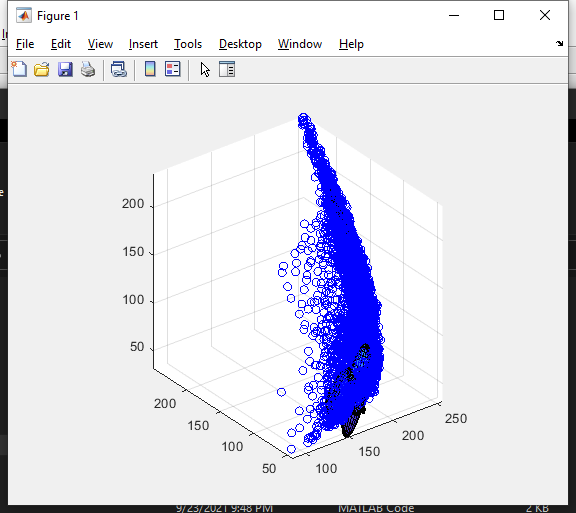
\includegraphics[scale = 0.6]{GMM.png}
    \item There are two processes in short
        \begin{enumerate}
            \item Initialization: The mean was calculated at random using the matlab function rand. Covariance initialization was a little more difficult because it had to be positive semi definite. As a result, it was merely initialized by computing the cov of all the images(pixels x 3 dimension), elements, and ensuring that it was PSD and that its inverse existed.
            \item Number of gaussians in GMM: When it comes to the number of gaussians, there is an optimal number.The number of gaussians in our sample was fixed to seven. We can't fully capture the color space if the number of gaussians is low, so our method underfits and the accuracy is low. On the other hand, if the number of gaussians is increased, the algorithm tends to overfit, which may not be a good generalization. Overfitting will lead to poor prediction.
        \end{enumerate}
        
\end{itemize}
\section{Train Data }
    \begin{itemize}
        \item The same procedure is used to begin training and collect orange pixels as with a single gaussian. To get a rough idea of where the ball was, we employed the iterative technique of Maximum Likelihood Estimation. 
        \item Covariance was set to the covariance of the orange pixels, while mu and pi were set to random values using MATLAB's rand function. Although not fully random as described in the project description, it was sufficiently random for its purpose and ensured a square, PSD matrix. 
        \item We thought starting with the estimating stage and then alternated till we reached our pre-determined threshold. That could be a really good idea to achieve
    \end{itemize}
\section{Test Data}
    \item The normal process stated in the standards is followed when predicting from test results.The expected image, like Single Gaussian, is binary, with orange representing white and the rest being black. Each image is returned after being added to a cluster described by a cell array to allow for various sizes.
\section{Distance}
    \item The distance was implemented by first saving the predicted images of a GMM run (K = 8, threshold value = 0.000008) Once this was done,  regionprops were used to find the largest circle in any image that could have a radius of  to describe an area. A grade 4 model could then be fitted from  of the surfaces found to the distances (which are available in the file names of the training images) (MATLAB Polyfit). Finally,  GMM fed the predicted images of the test set into a similar algorithm. As with the previous "training", they were manipulated and circles were found. The area of all these circles was then inserted into the coefficients to estimate a distance 
    \begin{itemize}
        \item Distance of Ball Figure 1: 225.7899
        \item Distance of Ball Figure 2: 245.9386
        \item Distance of Ball Figure 3: 222.3892
        \item Distance of Ball Figure 4: 58.3664
        \item Distance of Ball Figure 5: 130.1384
        \item Distance of Ball Figure 6: 191.6834
        \item Distance of Ball Figure 7: 231.1142
        \item Distance of Ball Figure 8: 240.7131

    \end{itemize}

    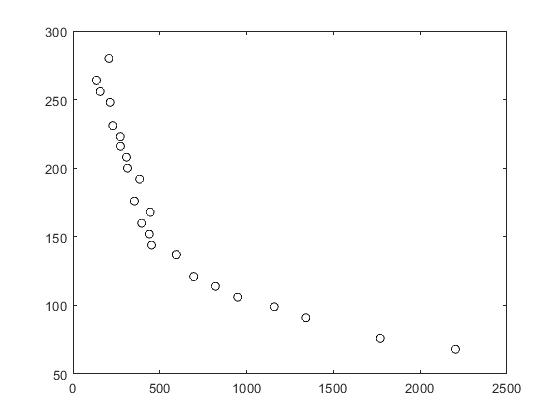
\includegraphics[scale = 0.6]{polyfitForMeasureDepth.jpg}
    
    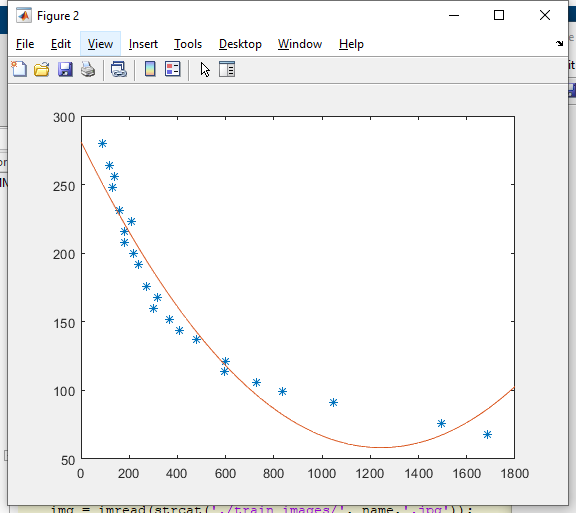
\includegraphics[scale = 0.6]{distance fit.png}
    
\section{Conclusion}
It is hard to survey the nature of GMM. The outcomes from test pictures 4-8 were discernibly better compared to SG, as the features and shadows were all the more precisely anticipated. For certain pictures, the ball was predominantly perceived and picture 1 was properly without a ball. The calculation actually battled with test pictures 2-3, in any case. We accept that this was to do with the lighting and picture qualitycontrasts in these two pictures. Regardless of whether the shading space or absence of handling to battle this, GMM couldn't perceive the ball with an alternate point. At the day's end, GMM is just K single gaussians. It isn't definitively more safe to these issues, just K-1 additional shadings.
\end{document}
